% ****** Start of file aipsamp.tex ******
%
%   This file is part of the AIP files in the AIP distribution for REVTeX 4.
%   Version 4.1 of REVTeX, October 2009
%
%   Copyright (c) 2009 American Institute of Physics.
%
%   See the AIP README file for restrictions and more information.
%
% TeX'ing this file requires that you have AMS-LaTeX 2.0 installed
% as well as the rest of the prerequisites for REVTeX 4.1
%
% It also requires running BibTeX. The commands are as follows:
%
%  1)  latex  aipsamp
%  2)  bibtex aipsamp
%  3)  latex  aipsamp
%  4)  latex  aipsamp
%
% Use this file as a source of example code for your aip document.
% Use the file aiptemplate.tex as a template for your document.
\documentclass[%
 aip,jap,
% jmp,
% bmf,
% sd,
% rsi,
 amsmath,amssymb,
%preprint,%
 reprint,%
% floatfix,
%author-year,%
%author-numerical,%
% Conference Proceedings
]{revtex4-1}

\usepackage{graphicx}% Include figure files
\usepackage{dcolumn}% Align table columns on decimal point
\usepackage{bm}% bold math
%\usepackage[mathlines]{lineno}% Enable numbering of text and display math
%\linenumbers\relax % Commence numbering lines

\usepackage[utf8]{inputenc}
\usepackage[T1]{fontenc}
\usepackage{mathptmx}
\usepackage{etoolbox}
\usepackage{multirow}

%% Apr 2021: AIP requests that the corresponding
%% email to be moved after the affiliations
\makeatletter
\def\@email#1#2{%
 \endgroup
 \patchcmd{\titleblock@produce}
  {\frontmatter@RRAPformat}
  {\frontmatter@RRAPformat{\produce@RRAP{*#1\href{mailto:#2}{#2}}}\frontmatter@RRAPformat}
  {}{}
}%
\makeatother
\begin{document}


\title[]{Microwave induced transformation of defect in SiC and GaAs}
\author{O. Olikh}
 \email{olegolikh@knu.ua}
 \affiliation{Physics Faculty, Taras Shevchenko National University of Kyiv, Kyiv 01601, Ukraine}%Lines break automatically or can be forced with \\
\author{P. Lytvyn}%
\affiliation{
V. Lashkaryov Institute of Semiconductor Physics of NAS of Ukraine, Kyiv 03028, Ukraine%\\This line break forced with \textbackslash\textbackslash
}%

\date{\today}% It is always \today, today,
             %  but any date may be explicitly specified

\begin{abstract}
The influence of microwave radiation (2.45~GHz, 1.5~W/cm$^2$, up to 80~s) on defects was studied in single crystals $n$-6H–SiC, $n$-GaAs and epi-GaAs.
The capture cross-section of charge carrier have been found to change
and defect complexes to be reconstructed due to the growing number of  interstitial atoms in the near surface layer.
The correlation between the changes in defect sub-system and deformation of the near surface layer is analyzed.
The possible mechanisms of the revealed effects are discussed.
\end{abstract}


\maketitle


\section{\label{sec:Int}INTRODUCTION}

Microelectronics is a field of primary importance today, and the investigation of how semiconductors and their structure properties change under the action of various external factors has become one of the most important tasks in material science.
A great number of theoretical and experimental researches have been aimed at revealing degradation mechanisms in microelectronic devices and developing new technologies of their production.
The influence of certain factors, for example, radiation, has been studied quite well ---- see, for instance, Refs.~\onlinecite{KozlovsEn,RadiationEffectsBook,DefByIon}.
At the same time, new agents begin to attract more attention, such as ultrasound loading\cite{Olikh2018JAP,Olikh2006TPL} (USL),
or microwave treatment\cite{MW:Rev,ZOHM2000,BHUNIA1998,Bacherikov2003En,Pashkov1994En,
BoltovetsEn,Milenin1994En,BelyaevIntac,ASHKINADZE1996,ProcSPIE,Belyaev1998JTFEn,
Bacherikov2008En,Konakova2015En,Konakova2012FTPEn}) (MWT).
As for MWT, the superhigh frequency (SHF) electromagnetic radiation has found a wide application due to its capability to heat solid bodies\cite{MW:Rev,ZOHM2000}.
This approach is peculiar because of its high efficiency, capability to increase the temperature
of a sample as a whole or at chosen locations with extremely high speeds of heating\cite{MW:Rev}.
As a result, MWT is widely used to synthesize various compounds, semiconducting compounds including.\cite{MW:Rev,BHUNIA1998})
However, this kind of external influence also causes the change in various characteristics of semiconductor materials and device structures.
For instance, it has been found that irradiation by  SHF causes the relaxation of internal stresses and modification of near surface regions
in GaAs and InP structures, \cite{BoltovetsEn,Pashkov1994En,Milenin1994En,BelyaevIntac,ProcSPIE,Konakova2015En,Konakova2012FTPEn}
the leveling of surface microrelief in SiC/SiO$_2$ structures,\cite{Bacherikov2003En}
redistribution of impurities\cite{Bacherikov2003En,Belyaev1998JTFEn,Konakova2015En}
and change in charge state in the complexes\cite{Milenin1994En} as well as generation of defects \cite{Belyaev1998JTFEn}.
One of the consequences the structure-admixture ordering  lead to is the decrease in the range of
Schottky diode parameter spread.\cite{Milenin1994En},\cite{Belyaev1998JTFEn}
Moreover, MWT has been found to induce changes in the properties of Ti, Gd and Er films deposited on silicon carbide,\cite{Bacherikov2008En},
as well as reconstruction of GaAs photoluminescence spectra, \cite{BelyaevIntac,ProcSPIE,Belyaev1998JTFEn}
the peculiarities of the effect being dependent both on the type of dopant and crystal structure orientation of the samples.
As a whole, these facts allow us to consider MWT as one of the most promising ways of modifying semiconductor devices.

On the other hand, it is of wide knowledge that the properties of semiconductor structures are determined very much by their defect subsystem.
In fact, the defects in SiC and GaAs are under active investigation up to now.
\cite{SiCDavid,SiCWei,GAPel2020,GASobolev2020}
At the same time,
the more detailed information about how MWT influences deep center parameters is practically unknown.
The aim of our work is to investigate MWT impact on the parameters of deep centers located in the near surface region of $n$–-6H-–SiC and $n$-–GaAs single crystals,
as well as on  GaAs  epitaxial structures by means of acoustoelectric  transient spectroscopy.

\section{\label{sec:Exp}EXPERIMENTAL DETAILS}

It has been reported \cite{BoltovetsEn,Milenin1994En,BelyaevIntac,ASHKINADZE1996,ProcSPIE} that generally,
the MWT impact on semiconductor structures depends on many factors.
The main of them are the initial level of structural perfectness, conductivity, dielectric permittivity and structure topology.
In order to estimate how MWT affects the defect parameters we chose different samples in view of doping degree, initial level of residual mechanical stress as well as structure.
They were as follows.

\noindent
i)~Single crystal $n$--6$H$--SiC wafers, grown by Leli method and doped with nitrogen.
   The samples were:
    490~$\mu$m thick plates with dimensions $5\times10$~mm$^2$ and  carrier concentration $(3-6)\times10^{18}$~cm$^{-3}$
    (further on SIC1 and SIC2);
    and 460~$\mu$m thick wafer of the same dimensions with concentration of carriers $(1-3)\times10^{18}$~cm$^{-3}$ (SIC3).

\noindent
ii)~GaAs single crystal plates with thickness of 300~$\mu$m.
   The plates were (100) oriented, doped with tin, the concentration of electrons was $(1.5-2.5)\times10^{18}$~cm$^{-3}$
   for sample  GAS1 and $(3-5)\times10^{16}$~cm$^{-3}$ for sample GAS2.
   GAT denotation is used for wafer (111), which was doped by tellurium,  $n = (1-2)\times10^{18}$~cm$^{-3}$.

\noindent
iii)~Epitaxial $n$-$n^+$ structures of GaAs which were 300~$\mu$m thick single crystal substrates $n = 2 \times10^{18}$~cm$^{-3}$
   covered with 6~$\mu$m thick layer with carrier concentration $3.9\times10^{15}$~cm$^{-3}$
   (sample GAE1), $3.5\times10^{15}$~cm$^{-3}$ (GAE2),
   $5.0\times10^{15}$~cm$^{-3}$ (GAE3).
   The substrate and epitaxial layer were doped with tellurium.

\noindent
iv)~Epitaxial $n$-$n^+$-$n^{++}$ structures of GaAs:Te with a buffer layer.
 They were made from single crystal (100) substrate (300~$\mu$m, $n= 2\times10^{18}$~cm$^{-3}$)
  subsequently covered with 1~$\mu$m layer with $n=8\times10^{16}$~cm$^{-3}$ and
  2~$\mu$m layer with $n=7\times10^{15}$~cm$^{-3}$.
  Two samples (GAB1 and GAB) were cut from different wafers and used in the investigation.

Epitaxial systems were produced by the gas phase epitaxy technique.
The samples used in the experiment are categorized in Fig.~\ref{figSamp_TAV}.

\begin{figure}
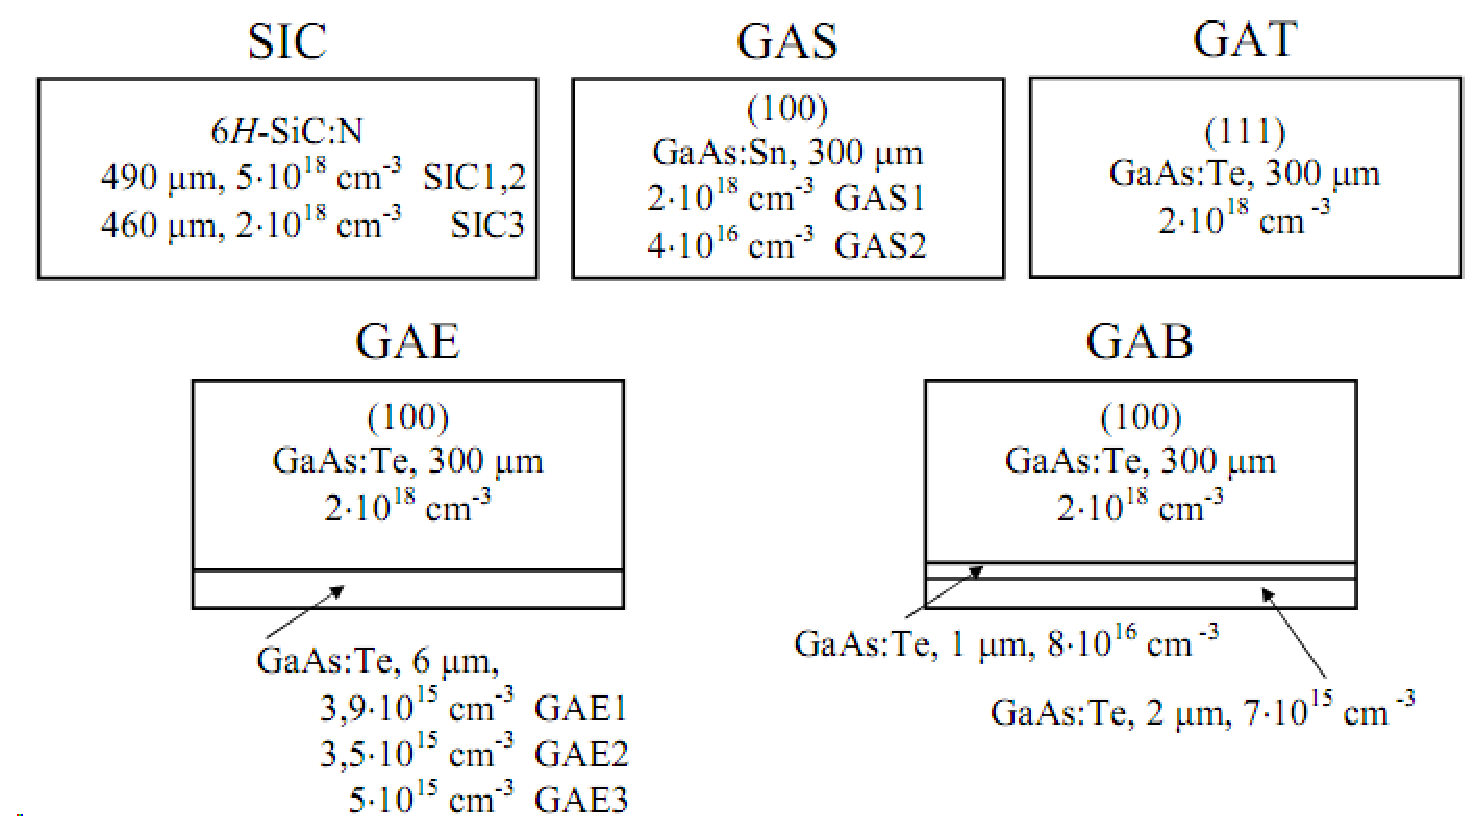
\includegraphics[width=0.5\textwidth]{Fig1}
\caption{\label{figSamp_TAV}
Structures for deep level investigations
}%
\end{figure}

MWT of the sample was carried out in free space at room temperature in the magnetron at the frequency of  $2.45$~GHz
and specific power $1.5$~W/cm$^{2}$.
The epitaxial structures were irradiated from the side of the epitaxial layer.
The total exposition time $t_\mathtt{MWT}$ varied in the range $20-80$~s for different samples.
To avoid essential heating, the maximum single irradiation exposure time was no more than  five seconds.


The parameters of deep centers, such as the efficient cross section of electron capture $\sigma_n$
and location of the center energy level with relation to conductivity band bottom $E_c-Et$ were determined before and after MWT.
For this purpose, we used acoustoelectric transient spectroscopy. \cite{OstrovPAN,OlikhSSC,PANnewEn,OstrovskiiSST}
The method is schematically presented in Fig.~\ref{figTAV}.
The samples were placed on the LiNbO3 piezoelectric plate in which acoustic waves were excited as impulses.
After ultrasound impulse termination, the relaxation of transverse acoustoelectric voltage (TAV) takes place according to the law
\begin{equation}\label{eqVtav}
  V_\mathtt{TAV}(t)=V_{\mathtt{TAV},0}\exp(-t/\tau).
\end{equation}

\begin{figure}
\includegraphics[width=0.5\textwidth]{fig2}
\caption{\label{figTAV}
Scheme of TAV signal  measurements.
Time dependence of radio impulse $V_\mathtt{RF}$ of ultrasound excitation in piezoelectric plate and the resulting TAV signal $V_\mathtt{TAV}$ are shown schematically
}%
\end{figure}

The simple exponential dependence according to Eq.~(\ref{eqVtav}) is observed in cases when only one type of deep centers is effective in acoustoelectric interactions.
For $n$-type semiconductor, the characteristic time of relaxation is described by equation \cite{OstrovPAN,OstrovskiiSST}
\begin{equation}\label{eqPANtau}
  \tau=\frac{1}{\sigma_n\,\upsilon_{\mathrm{th},n}\,N_c}\exp\left(\frac{E_c-E_t}{kT}\right),
\end{equation}
where
$\upsilon_{\mathrm{th},n}$ is the electron thermal velocity
$N_C$ is the densities of states in the conduction band.



The experimental measurements of the TAV relaxation at different temperatures and further approximation of the results according to Eq.~(\ref{eqVtav})
allowed us to obtain $\tau(T)$ dependence.
The $E_c-Et$ was determined from the slope of $\tau$ dependence on $(kT)^{-1}$ in semi-logarithmic scale
and then, by using Eq.~(\ref{eqPANtau}2), $\sigma_n$ was calculated.
The measurements were performed in the temperature range $(290-350)$~K except GAB samples,
the TAV for which was high enough to be measured only after heating to above 310~K.

For single crystal samples,  before and after MWT, we also determined curvature radius $R_\mathrm{cur}$
and deformation $\xi_\mathrm{cur}$ of near surface crystallographic planes.
The value of  $\xi_\mathrm{cur}$ was estimated by X-ray method from the change in the angle of diffraction
maximum location  during sample translation,\cite{Godwod}
the curvature was measured by the profilometer DekTak 3030 Veeco Instruments.
$R_\mathrm{cur}$ and $\xi_\mathrm{cur}$ were measured with a relative error no more than 2~\%.
For GaAs single crystals, we also analysed the distribution of structural defects over the area using the method of
Borman X-ray projection topography, and estimated the distribution of dislocation  densities and micro stresses from the
analysis of the intensities of Friedel reflection pairs $hkl$ and $hk$\emph{\={l}}.



\section{\label{sec:Rez}RESULTS AND DISCUSSION}

Fig.~\ref{figTauTAV} presents typical temperature dependences of $\tau$ for the samples before and after MWT.
The above data show the change not only in the curve slopes (which is directly related to the level location in the gap)
but also in the absolute value of  characteristic time of relaxation TAV that after MWT.
The character of the MWT impact (the decrease or increase in relaxation time) depends not only on exposition time and degree of doping but also on internal structure of the samples under study.
The obtained results are generalized in Table~\ref{tabMW}.
It is seen that in silicon carbide samples there are two deep levels, labeled ESC1 and ESC2, while in gallium arsenide, they are six (EGA1–EGA6).



\begin{figure*}
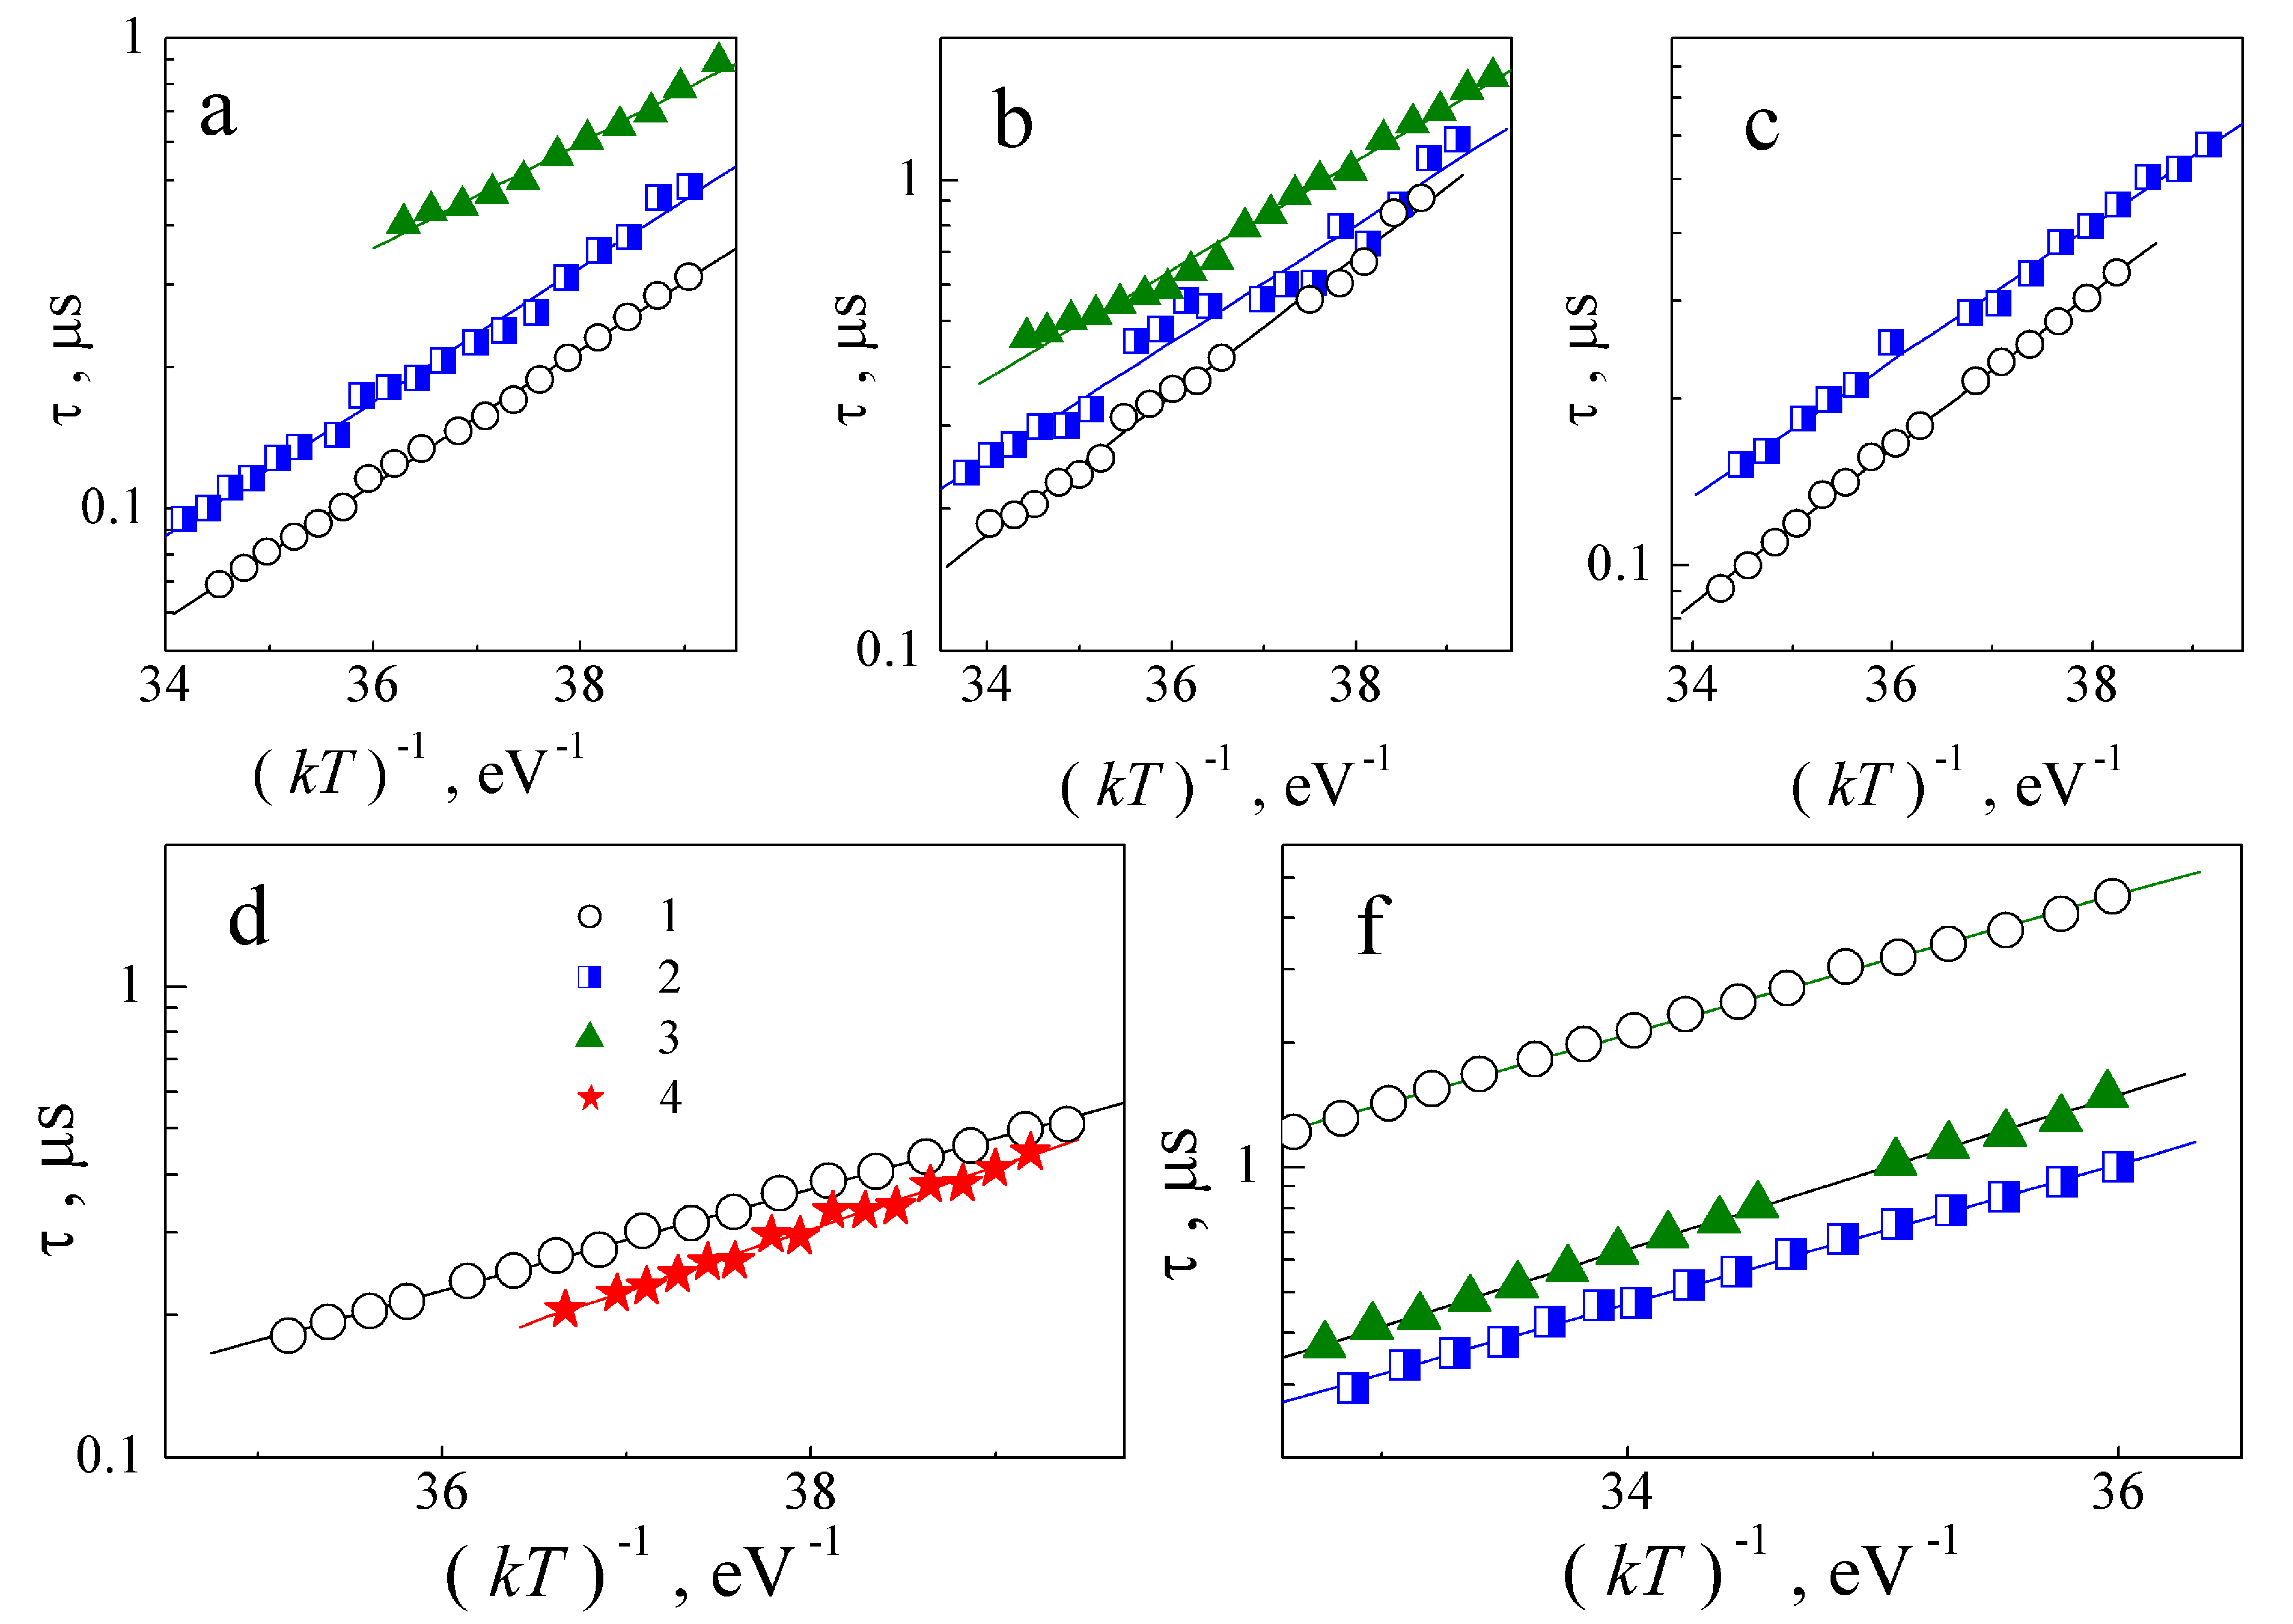
\includegraphics[width=0.7\textwidth]{Fig3}
\caption{\label{figTauTAV}
Dependences of TAV relaxation time on inverse temperature for samples SIC2 (a), SIC3 (b), GAS2 (c), GAE2 (d) and GAB1 (e) before and after MWT.
$t_\mathtt{MWT}$, s: 0 (curves 1), 20 (2), 40 (3), 60 (4)
}%
\end{figure*}




\begin{table*}
\caption{\label{tabMW}
The determined defect parameters in samples $n$--GaAs and $n$--6$H$--SiC
}
\begin{ruledtabular}
\begin{tabular}{ccccccc}
Sample& $t_\mathrm{MWT}$, s &Level &$(E_c-E_t)$, eV &$\sigma_n$, cm$^2$\textsuperscript{ a)}&$R_\mathrm{cur}$, m&$\xi_\mathrm{cur}$\\
%\midrule
\hline
SIC1& 0 &ESC1& $0.33\pm0.01$ &$(7\pm4)\cdot10^{-18}$&$\infty$&0\\ %\cline{2-7}
& 20 &ESC1& $0.33\pm0.01$ &$(5\pm3)\cdot10^{-19}$&170.2&$8.7\cdot10^{-7}$\\ %\cline{2-7}
& 40 &ESC2& $0.26\pm0.01$ &$(2\pm1)\cdot10^{-19}$&\multicolumn{2}{c}{\multirow{2}{*}{-}}\\ %\cline{2-5}
& 80 & \multicolumn{3}{c}{weak signal}&\multicolumn{2}{c}{}\\ %\hline
SIC2& 0 &ESC1& $0.33\pm0.01$ &$(7\pm4)\cdot10^{-18}$&$>2000$&$<1.2\cdot10^{-7}$\\ %\cline{2-7}
& 20 &ESC1& $0.33\pm0.01$ &$(5\pm3)\cdot10^{-19}$&171.9&$1.4\cdot10^{-6}$\\ %\hline
SIC3& 0 &ESC1& $0.34\pm0.02$ &$(3\pm2)\cdot10^{-18}$&3.8&$6.1\cdot10^{-5}$\\ %\cline{2-7}
& 20 &ESC2&$0.29\pm0.01$ &$(5\pm3)\cdot10^{-19}$&5.5&$4.2\cdot10^{-5}$\\ %\cline{2-7}
& 40 &ESC2& $0.26\pm0.01$ &$(10\pm7)\cdot10^{-20}$&\multicolumn{2}{c}{\multirow{2}{*}{-}}\\ %\cline{2-5}
& 80 &ESC2& $0.23\pm0.01$ &$(6\pm4)\cdot10^{-20}$&\multicolumn{2}{c}{}\\ %\hline
GAS1& 0 &EGA1& $0.32\pm0.02$ &$(3\pm2)\cdot10^{-17}$&-53.8&$-2.8\cdot10^{-6}$\\ %\cline{2-7}
& 20 &EGA1& $0.31\pm0.01$ &$(2\pm1)\cdot10^{-17}$&22.9&$6.5\cdot10^{-6}$\\ %\cline{2-7}
& 40 & \multicolumn{3}{c}{weak signal}&\multicolumn{2}{c}{-}\\ %\hline
GAS2& 0 &EGA1& $0.32\pm0.01$ &$(4\pm2)\cdot10^{-17}$&17.2&$8.7\cdot10^{-6}$\\ %\cline{2-7}
& 20 &EGA2& $0.28\pm0.01$ &$(5\pm2)\cdot10^{-18}$&14.7&$1.0\cdot10^{-5}$\\ %\cline{2-7}
& 40 & \multicolumn{3}{c}{weak signal}&\multicolumn{2}{c}{}\\ %\cline{1-5}
GAT& 0 &EGA3& $0.49\pm0.02$ &$(5\pm3)\cdot10^{-14}$&\multicolumn{2}{c}{}\\ %\cline{2-5}
& 20 &EGA4& $0.40\pm0.02$ &$(2\pm1)\cdot10^{-15}$&\multicolumn{2}{c}{}\\ %\cline{1-5}
GAE1& 0 &EGA5& $0.24\pm0.01$ &$(2\pm1)\cdot10^{-18}$&\multicolumn{2}{c}{}\\ %\cline{2-5}
& 60 &EGA2& $0.29\pm0.01$ &$(10\pm6)\cdot10^{-18}$&\multicolumn{2}{c}{}\\ %\cline{1-5}
GAE2& 0 &EGA5& $0.25\pm0.01$ &$(2\pm1)\cdot10^{-18}$&\multicolumn{2}{c}{}\\ %\cline{2-5}
& 60 &EGA2& $0.30\pm0.01$ &$(2\pm1)\cdot10^{-17}$&\multicolumn{2}{c}{}\\ %\cline{1-5}
GAE3& 0 &EGA6& $0.43\pm0.01$ &$(8\pm5)\cdot10^{-17}$&\multicolumn{2}{c}{-}\\ %\cline{2-5}
& 60 &EGA6& $0.46\pm0.02$ &$(7\pm4)\cdot10^{-16}$&\multicolumn{2}{c}{}\\ %\cline{1-5}
GAB1& 0 &EGA4& $0.39\pm0.01$ &$(10\pm7)\cdot10^{-18}$&\multicolumn{2}{c}{}\\ %\cline{2-5}
& 20 &EGA4& $0.39\pm0.01$ &$(4\pm2)\cdot10^{-17}$&\multicolumn{2}{c}{}\\ %\cline{2-5}
& 40 &EGA6& $0.43\pm0.02$ &$(10\pm6)\cdot10^{-17}$&\multicolumn{2}{c}{}\\ %\cline{1-5}
GAB2& 0 &EGA4& $0.40\pm0.01$ &$(10\pm6)\cdot10^{-17}$&\multicolumn{2}{c}{}\\ %\cline{2-5}
& 20 &EGA4& $0.41\pm0.01$ &$(10\pm6)\cdot10^{-17}$&\multicolumn{2}{c}{}\\ %\cline{2-5}
& 40 &EGA6& $0.45\pm0.02$ &$(4\pm2)\cdot10^{-16}$&\multicolumn{2}{c}{}\\  %\hline
\multicolumn{6}{l}{\textsuperscript{ a)} \emph{at $T=300$~K for SIC, GA, GAE and at $T=340$~K for GAB}}\\
\end{tabular}
\end{ruledtabular}
\end{table*}

The presented data show a number of characteristic features:

\noindent
i)~The value of the carrier capture cross-section is much more sensitive to MWT than the energy location of the levels.
For example, $\sigma_n$ was found to change by an order of magnitude while the level location displacement was no more than 20\%;
moreover, the capture cross-section was modified at lower exposition times:
for instance, the value of $(E_c-E_t)$ for GAB1 practically did not change after 20~s MW exposition, while $\sigma_n$ grew about four times.

\noindent
ii)~In single crystals, the  MWT induced changes become stronger as the free charge carrier concentration decreases
(see data on samples GAS1 and GAS2) and the relative deformation increases (the increase of surface curvature).

\noindent
iii)~After durable MWT of single crystal samples ($t_\mathrm{MWT}>40$~s for GaAs,  $t_\mathrm{MWT}>80$~s for SiC),
TAV signal essentially decreases.
This fact correlates with the data  from,\cite{Belyaev1998JTFEn}
where it is reported about  the decreased concentration of the centers with levels in the upper half of the band gap in the result of MW annealing.

\noindent
iv)~The irradiation dose required to change essentially the parameters of the centers in epitaxial structures is higher than that for single crystal samples.
In particular, Table~\ref{tabMW} provides  data for the samples of GA and GAB series after 20~s MWT
that support this fact.
It should be noted that the doping level of  GAB and GAE substrates was the same as that of samples GAS1 and GAT,
the doping level of GAB epitaxial layer was similar to GAS2.
In addition, GAB, GAE and GAT contained the same doping impurity.
Thus, the found differences are determined by the structure of the samples, but not by the difference of their conductivities.

\noindent
v)~The character of changes in single crystal wafers and epitaxial structures is opposite:
for SIC, GAS, GAT, $\sigma_n$ and $(E_c-E_t)$ were found to decrease after MWT,
while for GAE and GAB both parameters increase.

We shall now consider the possible configuration of the centers discovered in the structures under study.
For this purpose we should take into account that the reported data for the trap main parameters vary in a wide range,
in particular the difference between the values of capture cross-sections can be as big as four orders of magnitude.\cite{Pavlovic2000}
One of the possible reasons of such a big spread can be an essential dependence
of thermal charge emission speed on  the electric field strength\cite{Bulyarskii2000,Makram} caused by
a)~decrease of ionization energy due to Pool--Frenkel effect or, for example, Coulombic interactions of centers \cite{Stellmacher};
b)~change of $\sigma_n$  value.\cite{Bourgoin2001}
As a rule, the change in $(E_c-E_t)$ comprises several hundredth of eV and
the change in capture cross-section reaches several orders of magnitude:
for instance, according to Bourgoin and Angelis\cite{Bourgoin2001}, at room temperature,
$\sigma_n$  for $EL2$ center in GaAs decreases 200 times
at intensity of $10^5$~V/cm.
As a result, the different methods used for investigating defects yield essentially different parameters for the same centers.
As an example, we can compare, from the reviews on various traps in gallium arsenide,
the data  obtained by methods of deep level transient spectroscopy \cite{Bourgoin:GaAs}
and thermally stimulated current.\cite{Pavlovic2000}
The data were obtained for the defects with closely located levels and very different values of capture cross-section.
Generalising the above said, we should note that it is the energy location of traps that we shall be oriented toward in our research.


The position of ESC1 level ($E_c-(0.33-0.34)$~eV) observed in the initial crystals of silicon carbide can be compared
with the position of $S$--center ($E_c-0.35$~eV) \cite{Lebed1999En,Anikin1991:2En,Anikin1991:3En},
EK–center ($E_c-0.34$~eV)\cite{Kuznets1997En}
or $(-/+)$ level center $E1$ ($E_c-0.34$~eV).\cite{Lebed1999En}
$S$--center is responsible for non-radiative recombination and
in 6$H$–SiC it is a self-interstitial defect.\cite{Lebed1999En})
According to the results reported in Refs.~\onlinecite{Anikin1991:2En,Anikin1991:3En},
$S$--center and $R$--center ($E_c-1,27$~eV) are associated with two different charge states
of one and the same defect,
while according to Lebedev~\emph{et al}.,\cite{Lebedev2000En}
$R$--center is a divacancy $\mathrm{V}_\mathrm{Si}\mathrm{V}_\mathrm{C}$.
It would be noted that  divacancy is a typical defect in 6$H$--SiC.\cite{SiCBaran,SiCDavid}
On the other hand, the level $E_c-0.39$~eV is more often associated with center $E1$.\cite{SiCWei,SiCKoizumi}
Thus, in our opinion, the ESC1 level is related to the  complex $\mathrm{V}_\mathrm{Si}\mathrm{V}_\mathrm{C}$.

After MWT, the position of the level responsible for TAV generation in SiC moves
to $E_c-(0.26-0.29)$~eV (level ESC2).
And this situation is also ambiguous: closely located are donor level $(0/+)$ of
center $E1$ ($E_c-(0.27-0.28)$~eV,\cite{Hemmingsson}
$E_c-0.26$~eV \cite{SiCWei,SiCKoizumi})
and center $X1$ ($E_c-0.3$~eV \cite{Lebedev2001En}).
The authors of the latter publication report about the essential dependence of $X1$ concentration on the crystal structural perfection.
They stress that this center is not identical to center $E1$.
In turn, the level $E1$ have been identified as the center of negative
correlation energy \cite{Lebedev2001En,SiCWei}
and dominating intrinsic point defect in $n$--type 6$H$--SiC.\cite{SiCSasaki}
According to Refs.~\onlinecite{SiCSasaki,SiCWei}, $E1$ is related to the carbon vacancy.
Taking into account the difference between $X1$ and ESC2 energy locations,
the configuration $\mathrm{V}_\mathrm{C}$ was associated with ESC2 level by us.


The data for every of the levels revealed in gallium arsenide are given in Table~\ref{tabEGA1}.
The presented data show that the centers are associated with intrinsic vacancy-related defects.



%\begin{longtable}{cccccc}
\begin{table*}
\caption{\label{tabEGA1}
Data reported for the levels close to detected levels
}
%\renewcommand{\arraystretch}{0.65}
\begin{ruledtabular}
\begin{tabular}{cccccc}
$(E_c-E_t)$, eV &$\sigma_n$, cm$^2$&configuration&method$\textsuperscript{ a)}$&epi--structure&Reference\\
\hline
\multicolumn{6}{c}{EGA1, ($E_c-E_t)=(0.31-0.32)$~eV}\\
0.33&-&complex with V$_\mathrm{As}$&DLTS&no&\onlinecite{EL6:Richter}\\% \hline
0.33&-&-&DLTS&no&\onlinecite{Neild1991}\\ %\hline
$0.31\div0.33$&-&V$_\mathrm{As}$&LDA&no&\onlinecite{EL6:Schultz}\\ %\hline
0.33&$1\cdot10^{-17}$&-&TSC&no&\onlinecite{Pavlovic2000}\\ %\hline
0.323&$1\cdot10^{-14}$&-&DLTS&yes&\onlinecite{Yousefi1995}\\ %\hline
0.334&$2\cdot10^{-15}$&&DLTS&yes&\onlinecite{Yousefi1995}\\ %\hline
0.35&-&complex with V$_\mathrm{As}$&PA&no&\onlinecite{EL6:Kuisma}\\ %\hline
$0.315\div0.325$&$3\cdot10^{-17}$&-&TSC&no&\onlinecite{Pavlovic:GaAs}\\ %\hline
0.33&-&-&TSC&no&\onlinecite{Tomozane:GaAs}\\ %\hline
$0.30\div0.33$&-&-&DLTS&no&\onlinecite{Lang:GaAs}\\ %\hline
\multicolumn{6}{c}{EGA2, ($E_c-E_t)=(0.28\div0.30)$~eV}\\
0.28&$5\cdot10^{-18}$&V$_\mathrm{As}$As$_i$&TSC&no&\onlinecite{Pavlovic2000}\\ %\hline
0.26&$3.5\cdot10^{-15}$&-&DLTS&yes&\onlinecite{Yousefi1995}\\ %\hline
%0.277&$5\cdot10^{-17}$&-&TSC&no&\onlinecite{Pavlovic:GaAs}\\ %\hline
0.30&-&intrinsic&DLTS&no&\onlinecite{PhysRevB1986}\\ %\hline
0.284&$1\cdot10^{-17}$&-&TSC&no&\onlinecite{Pavlovic:GaAs}\\ %\hline
0.28&-&intrinsic&TP&no&\onlinecite{Abele:GaAs}\\ %\hline
0.28&$8\cdot10^{-15}$&-&DLTS&yes&\onlinecite{Mircea1975}\\ %\hline
0.30&-&complex with Te&DLTS&no&\onlinecite{KolFTP1994En}\\ %\hline
0.30&$6\cdot10^{-15}$&V$_\mathrm{As}$As$_i$&DLTS&no&\onlinecite{Pons}\\ %\hline
\multicolumn{6}{c}{EGA3, ($E_c-E_t)=0.49$~eV}\\
0.50&-&Sb$_\mathrm{Ga}$&DLTS&no&\onlinecite{Samoilov1994En}\\ %\hline
0.48&$4\cdot10^{-16}$&As$_\mathrm{Ga}^{++}$&TSC&no&\onlinecite{Pavlovic2000}\\ %\hline
0.485&$2\cdot10^{-16}$&-&TSC&no&\onlinecite{Pavlovic:GaAs}\\ %\hline
0.48&-&impurity&TP&no&\onlinecite{Abele:GaAs}\\ %\hline
%0.51&$1\cdot10^{-12}$&-&DLTS&no&\onlinecite{Martin1977}\\ %\hline
0.49&$2\cdot10^{-13}$&impurity+V$_\mathrm{As}$&DLTS&yes&\onlinecite{GaAsBlood}\\ %\hline
0.48&$3\cdot10^{-13}$&-&DLTS&no&\onlinecite{Lang:GaAs}\\ %\hline
0.50&$1\cdot10^{-15}$&V$_\mathrm{As}$, V$_\mathrm{Ga}$Ga$_i$V$_\mathrm{As}$ &DLTS&no&\onlinecite{Pons}\\
\multicolumn{6}{c}{EGA4, ($E_c-E_t)=(0.39-0.41)$~eV}\\
0.42&-&-&DLTS&no&\onlinecite{Neild1991}\\ %\hline
0.41&-&V$_\mathrm{Ga}$V$_\mathrm{As}$&DLTS&no&\onlinecite{Samoilov1994En}\\ %\hline
$0.39$&-&V$_\mathrm{Ga}$Ga$_\mathrm{As}$&TSC&no&\onlinecite{FANG1990}\\ %\hline
$0.41$&$2\cdot10^{-13}$&-&DLTS&yes&\onlinecite{Bourgoin:GaAs}\\ %\hline
0.40&-&-&SCRC&yes&\onlinecite{ASHBY:GaAs}\\ %\hline
0.37&$2\cdot10^{-14}$&-&DLTS&yes&\onlinecite{Fang:EL6}\\ %\hline
0.40&-&V$_\mathrm{Ga}$Ga$_\mathrm{As}$&DLTS&no&\onlinecite{VaitkusEn}\\ %\hline
0.387&$2\cdot10^{-14}$&-&DLTS&yes&\onlinecite{Yousefi1995}\\ %\hline
\multicolumn{6}{c}{EGA5, ($E_c-E_t)=(0.24-0.25)$~eV}\\
0.23&-&-&DLTS&no&\onlinecite{Neild1991}\\ %\hline
0.23&$2\cdot10^{-17}$&-&TSC&no&\onlinecite{Pavlovic2000}\\ %\hline
$0.22\div0.25$&$8\cdot10^{-19}$&-&TSC&no&\onlinecite{Lin:GaAs}\\ %\hline
$0.26$&-&complex with V$_\mathrm{Ga}$&TSC&no&\onlinecite{FANG1990}\\ %\hline
0.24&-&-&TSC&no&\onlinecite{Tomozane:GaAs}\\ %\hline
0.23&-&intrinsic&TP&no&\onlinecite{Abele:GaAs}\\ %\hline
0.23&-&V$_\mathrm{Ga}$V$_\mathrm{As}$&DLTS&no&\onlinecite{Morrow:EL17}\\ %\hline
0.23&$1\cdot10^{-14}$&V$_\mathrm{Ga}$V$_\mathrm{As}$&DLTS&no&\onlinecite{Bourgoin:GaAs}\\ %\hline
0.23&$7\cdot10^{-15}$&-&DLTS&yes&\onlinecite{Mircea1975}\\ %\hline
%0.22&$2\cdot10^{-15}$&-&DLTS&no&\onlinecite{Fang:EL6}\\ %\hline
0.236&$1\cdot10^{-16}$&complex with V$_\mathrm{As}$&DLTS&yes&\onlinecite{GaAsBlood}\\ %\hline
0.258&$4\cdot10^{-16}$&-&DLTS&yes&\onlinecite{Yousefi1995}\\ %\hline
\multicolumn{6}{c}{EGA6, ($E_c-E_t)=(0.43-0.46)$~eV}\\
0.44&$1\cdot10^{-14}$&V$_\mathrm{As}$As$_i$, V$_\mathrm{As}$&TSC&no&\onlinecite{Pavlovic2000}\\ %\hline
0.44&$9\cdot10^{-15}$&-&TSC&no&\onlinecite{Pavlovic:GaAs}\\ %\hline
\multirow{2}{*}{0.43}&\multirow{2}{*}{$7\cdot10^{-16}$}&\multirow{2}{*}{intrinsic}&\multirow{2}{*}{DLTS}&\multirow{2}{*}{yes}&\onlinecite{Lefevre1977}\\
&&&&&\onlinecite{Bourgoin:GaAs}\\
%0.43&$7\cdot10^{-16}$&intrinsic&DLTS&yes&\onlinecite{Lefevre1977} \onlinecite{Bourgoin:GaAs}\\ %\hline
0.44&$2\cdot10^{-15}$&complex with V$_\mathrm{As}$&DLTS&yes&\onlinecite{KolFTP1989En}\\ %\hline
\multicolumn{6}{l}{$\textsuperscript{ a)}$ \emph{DLTS --- deep level transient spectroscopy;
TSC --- thermally stimulated current; LDA --- local density approximation;}}\\
\multicolumn{6}{l}{ \emph{PA --- positron annihilation techniques;
TP --- photoinduced transient spectroscopy;
SCLC --- space charge limited current}}\\
\end{tabular}
\end{ruledtabular}
\end{table*}
%\end{longtable}

There are several factors that cause the trap parameters to change.
They are as follows.

\noindent
i)~Transformation of the defect complex due to decay, involvement of additional components, change in distance between the defect components, etc.

\noindent
ii)~Defect recharging.

\noindent
iii)~Changes in the trap environment, which can result, for instance, in modified strength of electric field around the defect.

\noindent
iv)~Increase in concentrations of the given type of defects:
for instance, it is reported in Ref.~\onlinecite{Stellmacher}  that the change in ionization energy is proportional to the cubic root of the defect concentration.

The analysis of the observed phenomenons should take into account
the probable mechanisms of microwave radiation impact on crystals.
In the first place, the effect of temperature increase should be analyzed.
It is believed that the structural modification in the result of MWT  is mostly caused by the change
in defect charge state and elastic stress fields arising in instantly heated defect regions.
However, these processes are known to become intensive at the increased free charge carrier concentrations,\cite{MW:Rev}
while in our case the effects weaken with the growth of $n$ (samples GAS1 and GAS2).
Moreover, the applied mode of irradiation did not imply long term continuous exposure to MW oscillations,
which reduced the heating of the structure as a whole.
On the other hand, numerous researches show that the observed effects of MWT cannot be explained only by the mechanisms of fast  annealing,
so non-thermal factors should be considered as well.
In the recent research, more attention has been paid to non-thermal mechanisms of MWT action
(see, for example Ref.~\onlinecite{MW:Si2018} and the references it contains)
which cause dislocation generations and result in smaller  clusters of point defects in semiconductor wafers,\cite{Konakova2007JTFEn}
or even trigger recrystallization processes.\cite{MW:Si2018}
The possible non-thermal processes causing changes in structural characteristics of binary semiconductors were reported in Ref.~\onlinecite{Konakova2007JTFEn}.
In particular, the processes of dislocation oscillations under the action of electric field were analyzed,
and the decorating impurities have been found to influence essentially the behavior of dislocation segments.
On the one hand, the available impurities decrease the resonance frequency of oscillations
and provide the presence of electric charge,
on the other hand, at high oscillation amplitudes they can escape the dislocation,
which causes new chemical defects to arise.
In their turn, the point defects can perform superhigh frequency oscillations and diffuse in the result of MWT.

The found modifications of deep level parameters are the result of the above mentioned
structural reconstruction in semiconductor near surface regions  due to MWT.
The results of X--ray investigations show that MWT increases the convexity of single crystal samples,
which indicates the aggregation of interstitial defects in the near-surface layer,
in particular as a result of the generation of separate dislocations. \cite{BoltovetsEn,Konakova2012FTPEn}
Defect accumulation effect in the near surface region caused by MWT was reported in Refs.~\onlinecite{BoltovetsEn,Konakova2015En}.
To a certain extent, only SIC3 sample was an exclusion, but in this case rather strong deformation of near surface region was also observed prior to irradiation.
The researchers report \cite{Bacherikov2003En,Pashkov1994En,BoltovetsEn,Milenin1994En,BelyaevIntac} that in this stressed state,
MWT causes redistribution as well as certain weakening of elastic deformations, and this is what happens in SIC3.
The profilometry data correlate with the results from X-ray measurements.
The structure investigations show that
in the initial GaAs samples the density of dislocation has a W-like distribution over the plate area; the dislocation density over the plate diameter varies from $2\cdot10^{4}$~cm$^{-2}$ to $2\cdot10^{5}$~cm$^{-2}$.
This inhomogeneity in dislocation density distribution is the evidence of considerably strong elastic deformations in the sample.

The performed analysis shows that ESC1 and ESC2 centers are complexes of carbon vacancies,
EGA1 is associated with V$_\mathrm{As}$,
and EGA3 — with V$_\mathrm{As}$ or  V$_\mathrm{Ga}$Ga$_i$V$_\mathrm{As}$ complex.
MWT stimulated diffusion of the point defects, which are mostly intrinsic interstitial atoms, results in trap modifications.
ESC1 center in silicon carbide turns into ESC2 under the influence of closely located interstitial silicon:

\begin{displaymath}
  \mathrm{V}_\mathrm{Si}\;\mathrm{V}_\mathrm{C}+\mathrm{Si}_{\,i} \rightarrow
   \mathrm{V}_\mathrm{C}\,.
\end{displaymath}

Further modification of ESC2 parameters in SIC3 is caused by the enhanced electric field of dislocation.
In the samples of GAS2 at $t_\mathrm{MWT}=20$~s,
V$_\mathrm{As}$ transforms into complex V$_\mathrm{As}$As$_i$
(EGA2 center)
due to increased number of interstitial atoms in the near-surface layer:
\begin{displaymath}
\mathrm{V}_\mathrm{As}+ \mathrm{As}_{\,i} \rightarrow \mathrm{V}_\mathrm{As}\;\mathrm{As}_{\,i}\,.
\end{displaymath}

The similar process in GAS1 is more complicated because of higher charge carrier concentration:
it is reported (\cite{ZOHM2000}) that with the growth of resistance the depth of microwave penetration grows
and thus, the volume from which defect gettering begins in the near-surface layer grows as well.
In addition, the cause of weak (in comparison with GAS2) influence of MWT on trap parameters in GAS1 is the absence of pressure stresses,
which intensify MWT simulated complex formation process in the system’s intrinsic defects.
This consideration is supported by the data for silicon carbide single crystals.
In the GAT sample, which is also characterizes by a high concentration of free electrons,
transformation of EGA3 to EGA4 (V$_\mathrm{Ga}$Ga$_\mathrm{As}$ complex) is going on in the reaction described in Ref.~\onlinecite{FANG1990}:
\begin{displaymath}
  \mathrm{V}_\mathrm{Ga}\;\mathrm{Ga}_{\,i}\;\mathrm{V}_\mathrm{As}\rightarrow \mathrm{Ga}_\mathrm{Ga}\;\mathrm{V}_\mathrm{As}
  \rightarrow \mathrm{Ga}_\mathrm{As}\;\mathrm{V}_\mathrm{Ga}
\end{displaymath}


Accumulation of a great number of interstitial atoms in the near-surface layer at high doses of radiation
($t_\mathrm{MWT}\approx40$~s for gallium arsenide and $t_\mathrm{MWT}>80$~s for silicon carbide)
causes complete annihilation of vacancies (or transformation into antisite defects, whose levels are filled in the crystals with electron conductivity)
 and therefore TAV signal disappears (samples GAS1, GAS2, SIC1):
\begin{eqnarray}
  \nonumber
  \mathrm{SiC}&:&\mathrm{V}_\mathrm{Si}\;\mathrm{V}_\mathrm{Si}+\mathrm{Si}_{\,i}+ \mathrm{Si}_{\,i} \rightarrow 0\,;\\
  \nonumber
  \mathrm{GaAs}&:&\mathrm{V}_\mathrm{As}+\mathrm{As}_{\,i} \rightarrow 0\,;\quad
  \mathrm{V}_\mathrm{As}+\mathrm{Ga}_{\,i} \rightarrow \mathrm{Ga}_\mathrm{As}\,.
\end{eqnarray}

It is believed,\cite{OstrovskiiSST,OlikhSSC,OstrovPAN} that TAV
which arise in epitaxial structures
is mostly caused by the defects located on the epi--layer and substrate interface.
This difference in deep level location
is the cause of the difference between dose-dependent modification of defect parameters in epitaxial and single crystal samples.

In epitaxial structures $n$--$n^+$--GaAs and $n$--$n^+$--$n^{++}$--GaAs,
MWT induced increase of curvature radius reported in Refs.~\onlinecite{BoltovetsEn,Konakova2012FTPEn}
is the result of forming single dislocations and their further propagation deep into the structure along the glide planes.
As a result, the strength of both electric and stress field changes,
which causes defect transformation and thus the shift of respective deep levels.
As seen from Table~\ref{tabEGA1}, the levels of EGA5 and EGA6 are associated with complexes   V$_\mathrm{Ga}$V$_\mathrm{As}$  and V$_\mathrm{As}$As$_i$, respectively.
Such traps as EGA2 and EGA4 have also been found in epi-structures before. \cite{Yousefi1995,Mircea1975,Bourgoin:GaAs,ASHBY:GaAs,Fang:EL6,Lefevre1977,KolFTP1989En}
The observed MWT-stimulated transformations are caused by the growing number of interstitial atoms which are described by reactions like the following
\begin{displaymath}
  \mathrm{V}_\mathrm{Ga}\;\mathrm{V}_\mathrm{As}+\mathrm{Ga}_{\,i}+\mathrm{As}_{\,i} \rightarrow \mathrm{V}_\mathrm{As}\;\mathrm{As}_{\,i}
\end{displaymath}
for GAE1 and GAE2 and
\begin{displaymath}
  \mathrm{V}_\mathrm{Ga}\;\mathrm{Ga}_\mathrm{As}+\mathrm{As}_{\,i} \rightarrow
  \mathrm{Ga}_\mathrm{Ga}\;\mathrm{V}_\mathrm{As}+\mathrm{As}_{\,i} \rightarrow
  \mathrm{V}_\mathrm{As}\;\mathrm{As}_{\,i}
\end{displaymath}
for GAB1 and GAB2.
The increase in activation energy EGA6 in sample GAE3 is caused, most probably, by the change in
Coulombic interaction of interstitial--vacancy complexes
which is due to decrease in their concentration,
while the growth of capture cross-section EGA4 in GAB1 at $t_\mathrm{MWT}=20$~s
and EGA6 in GAE3 is associated with the growth of electric field strength caused by charged dislocations.


\section{CONCLUSION}
The influence of microwave radiation on the parameters of point defects (cross section of electron capture, energy levels in the gap)
was studied experimentally  in single crystals of $n$–-6$H$-–SiC and  $n$-–GaAs, as well as in gallium arsenide epitaxial structures.
The investigation shows that the traps available in the near-surface layer are associated with the intrinsic
vacancy-related defects.
The microwave radiation induced change of the trap energy level as well as capture cross section
is caused by the growing number of interstitial atoms in the near-surface layer.
The  radiation induced process involving the transformations of defect complexes are intensified in conditions of stresses.

\section*{Data Availability Statement}

The data that support the findings of this study are available from the corresponding author upon reasonable request.

\section*{References}

\bibliography{olikh}

\end{document}
